% !TeX program = xelatex
\documentclass[UTF8,a4paper,11pt,fontset=fandol]{ctexart}
\usepackage[margin=2.1cm]{geometry}
\usepackage{graphicx,xcolor,booktabs,tabularx,fancyhdr,caption,float}
\usepackage[colorlinks=true,urlcolor=blue!55!black,linkcolor=blue!55!black]{hyperref}
\definecolor{ink}{HTML}{304C5C}
\ctexset{section={format=\Large\bfseries\color{ink}},subsection={format=\normalsize\bfseries\color{ink}}}
\captionsetup{font=small,labelfont=bf,skip=6pt}
\setlength{\parindent}{2em}
\setlength{\parskip}{4pt}
\linespread{1.12}
\pagestyle{fancy}\fancyhf{}
\fancyhead[L]{\small 基于 Three.js 的四旋翼无人机建模（第二期）}
\fancyhead[R]{\small 建模实践记录}
\fancyfoot[C]{\small\thepage}
\setlength{\headheight}{15pt}
\title{\LARGE\bfseries 基于Three.js的四旋翼无人机建模(第二期)}
\author{朱华天 \quad GPT-6 Astra}
\date{2026年9月9日\\[7pt]{\small\url{https://github.com/ZHT1235456/Three-js-QUAV-by-Astra}}}
\begin{document}
\maketitle
\thispagestyle{plain}
\begin{abstract}
本文记录一次从生成式图像到可交互三维模型的实践：笔者先生成同一架四旋翼无人机的多视角参考图，再在 Codex 中与 GPT-6 Astra 对话，使用 Three.js 完成外观重建和细节迭代。结果包含机身、机臂、旋翼、电机、起落架与下挂云台，支持视角切换、结构分解和 GLB 导出。本文展示参考图与实测页面截图，并讨论航灯配色、建模实现和复现方法。
\end{abstract}

\section{从多视角图开始}
笔者首先使用新发布的 GPT-Image 2.5 生成了一架四旋翼无人机的多视角图，输入的提示词十分简洁：
\begin{quote}\color{ink}\bfseries
生成多张同一架旋翼无人机的不同视角图
\end{quote}
这里的图像工具名称与使用背景按笔者的实验记录叙述。最终选取的四张参考图分别展示透视、俯视、侧视和正视外观，保存在仓库的 \texttt{figures/} 中。它们共同确定了本次建模的视觉目标：深色碳纤维机身、X 形展开机臂、双叶旋翼、滑橇式起落架，以及机头下方的云台相机。

\begin{figure}[htbp]\centering
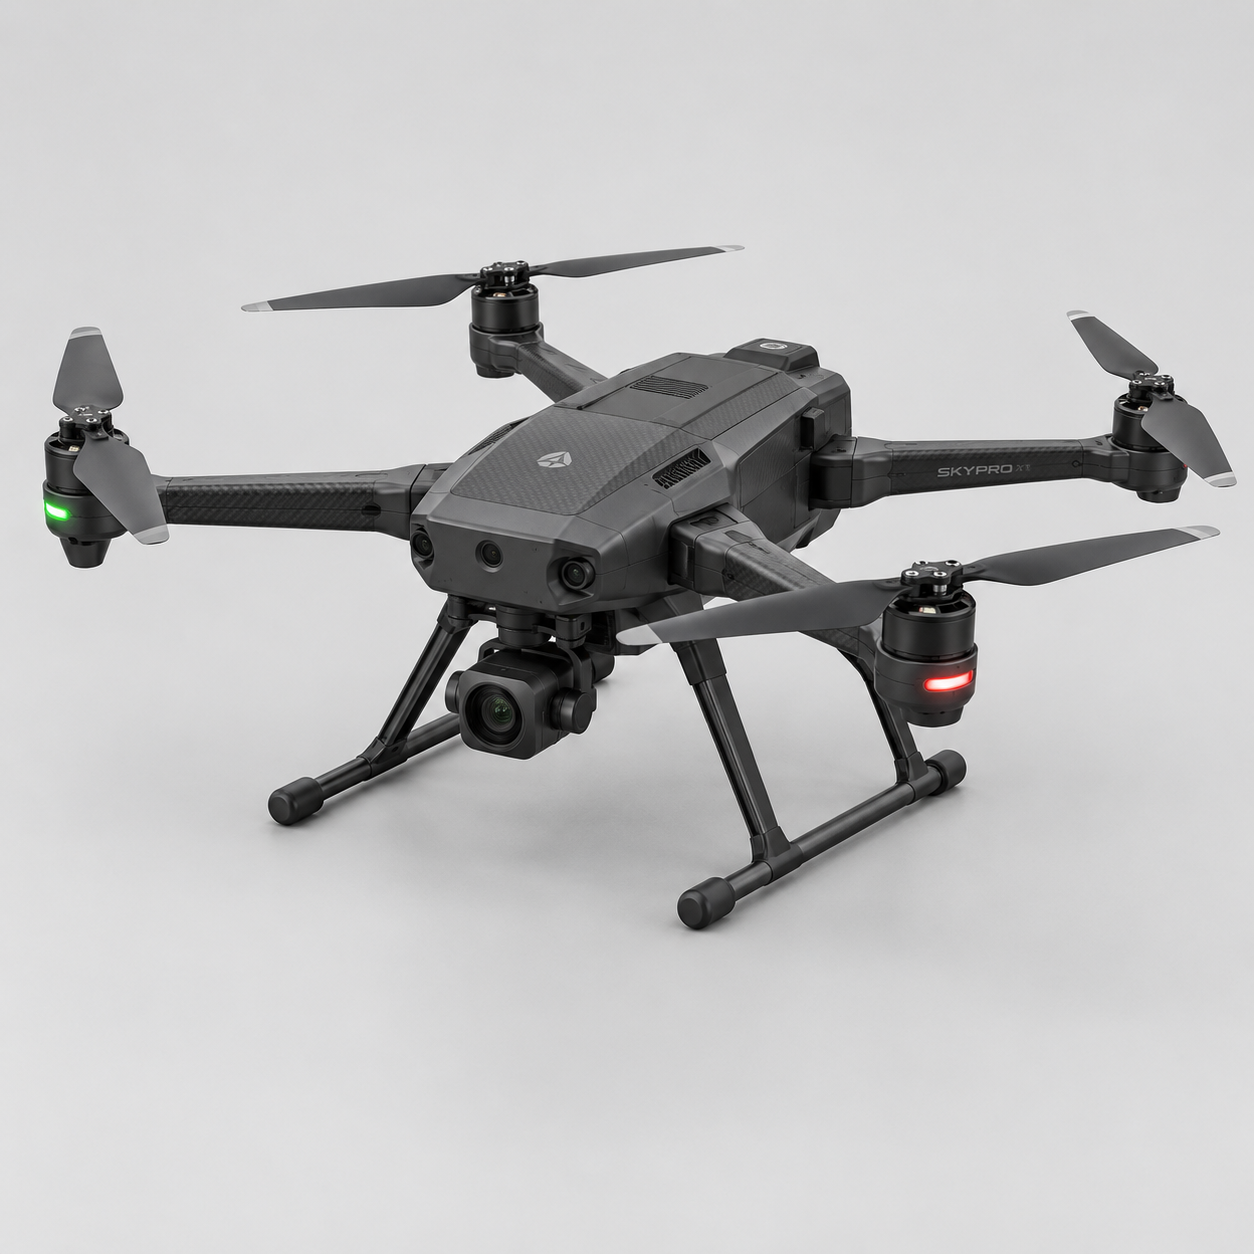
\includegraphics[width=.32\linewidth]{../figures/1.png}\hspace{.025\linewidth}
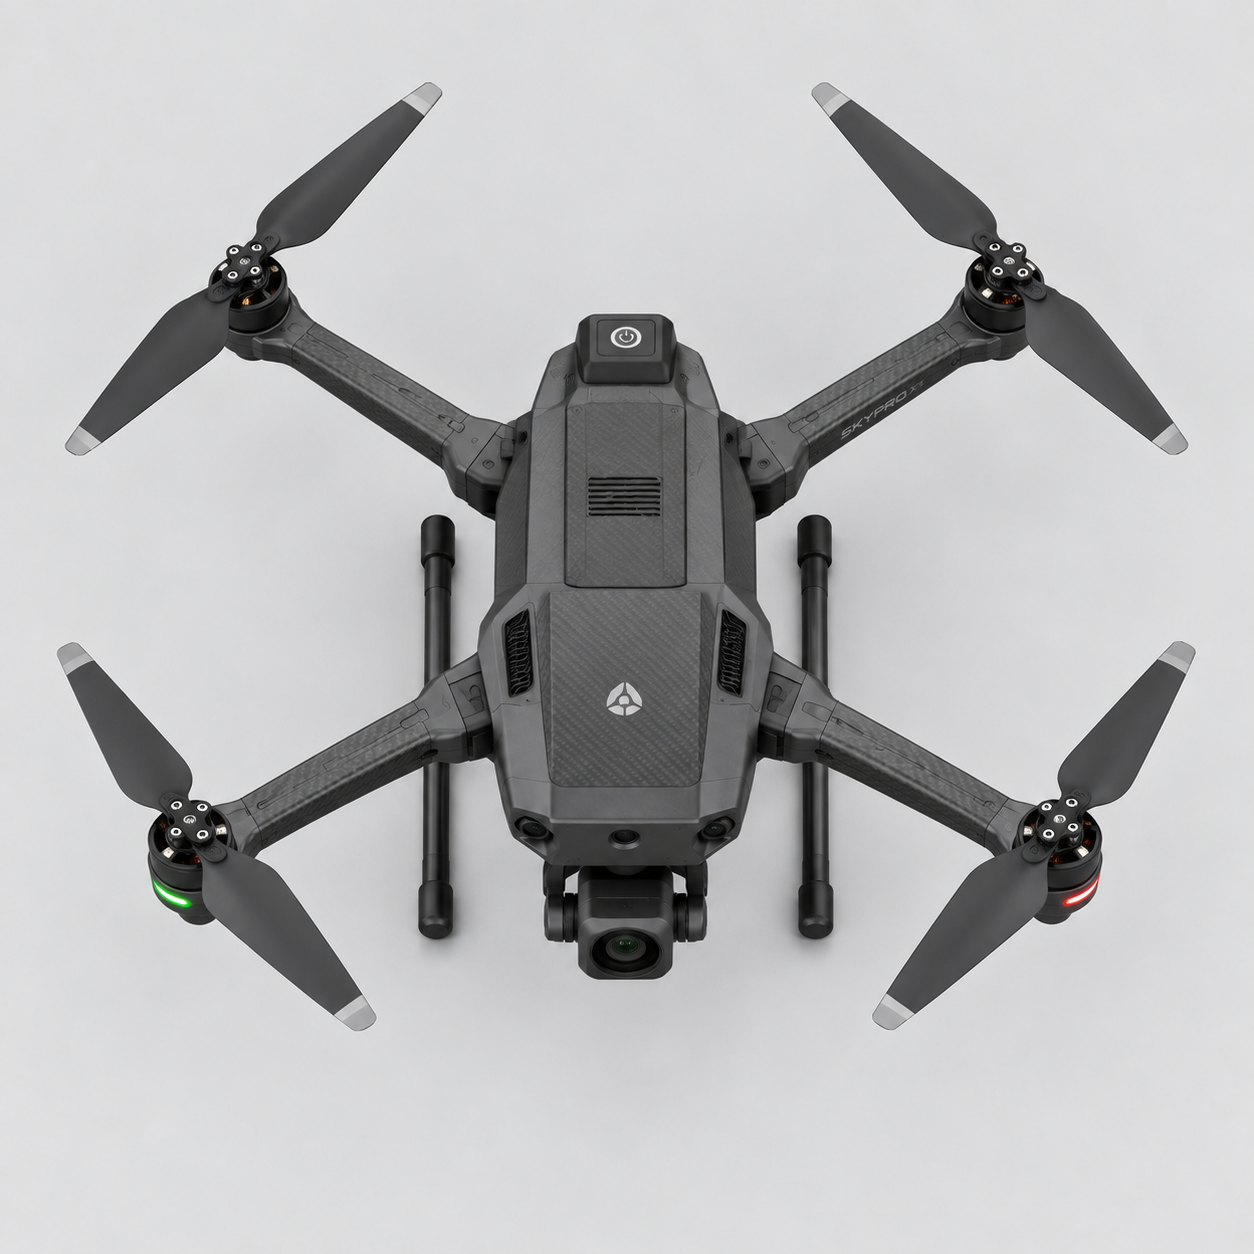
\includegraphics[width=.32\linewidth]{../figures/2.png}
\caption{生成的透视与俯视参考图。其他两个视角随项目一并公开。}
\end{figure}

\section{在 Codex 中完成建模}
随后，笔者在 Codex 中选择 GPT-6 Astra，将思考强度设为“轻度”，并提出“参考 figures，基于 three.js 建模”的要求。在初版基础上，经过三轮对话迭代，得到了令笔者非常惊艳的结果：不仅能在浏览器中自由观察整机，还能查看分解结构、转动旋翼并调整云台俯仰。下面的截图直接来自实际运行页面，展示的是可交互几何模型。

\clearpage
\section{建模效果：从整体到细节}
初版建立了整机结构，后续迭代逐步增加机身硬切面与壳体接缝、机臂套筒和螺钉、电机环带与通风槽、机身标识，以及镜头环、散热槽和云台线缆。桨叶进一步采用连续曲线轮廓和闭合截面，加入厚度、弯度、扭转及浅色桨尖。碳纤维纹理由程序生成，并叠加透明涂层材质。

\begin{figure}[H]\centering
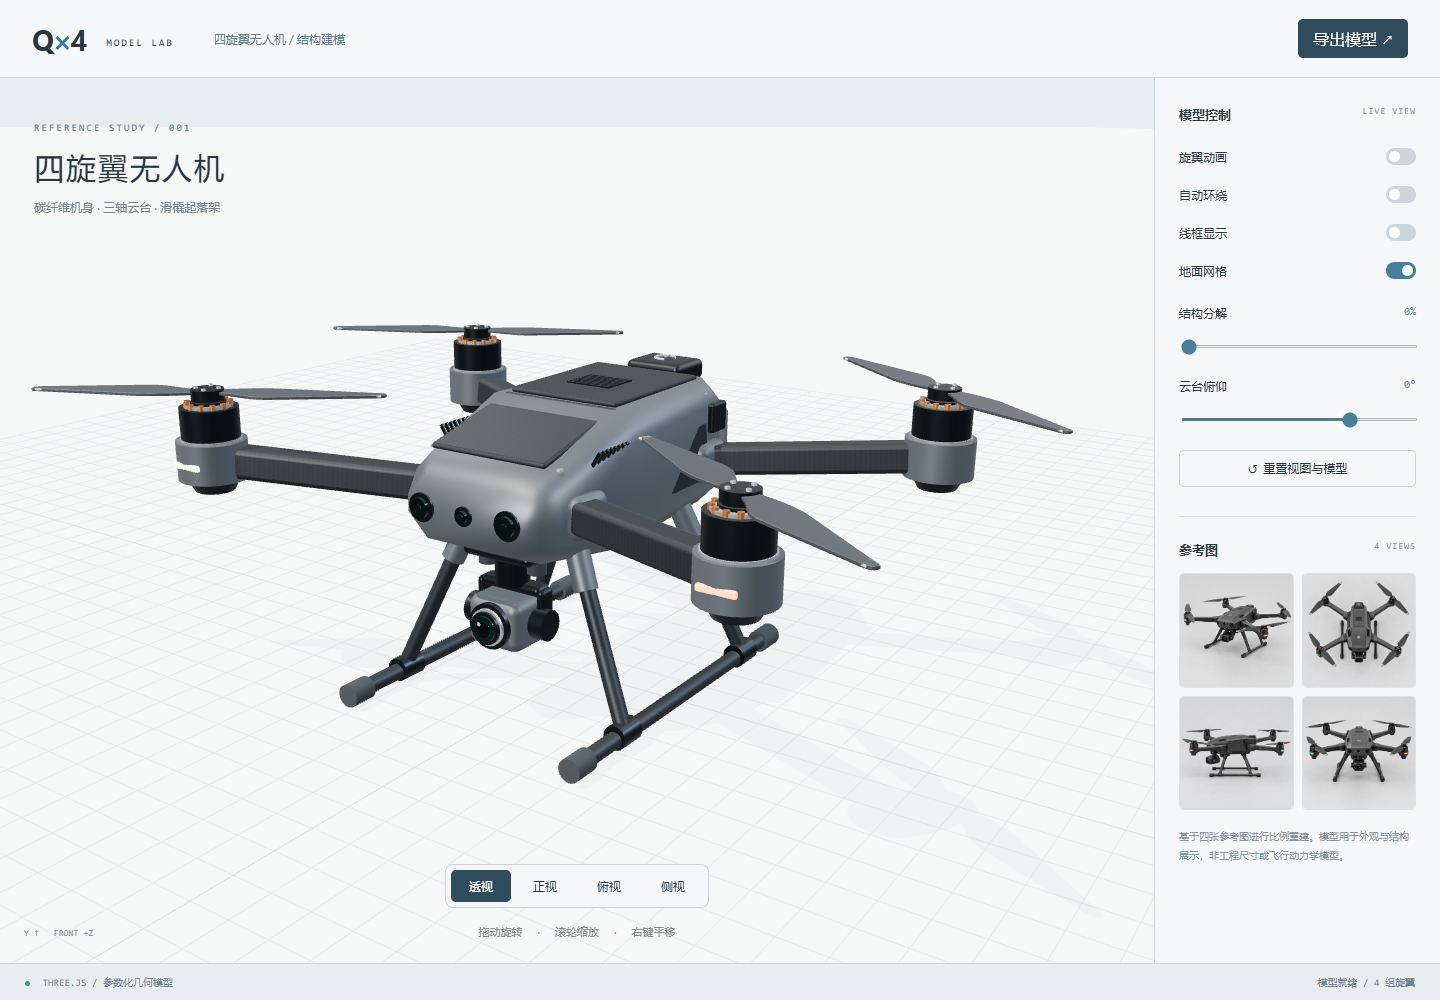
\includegraphics[width=.80\linewidth]{../preview.png}
\caption{透视效果截图：整机模型及右侧交互控制面板。}
\end{figure}
\begin{figure}[H]\centering
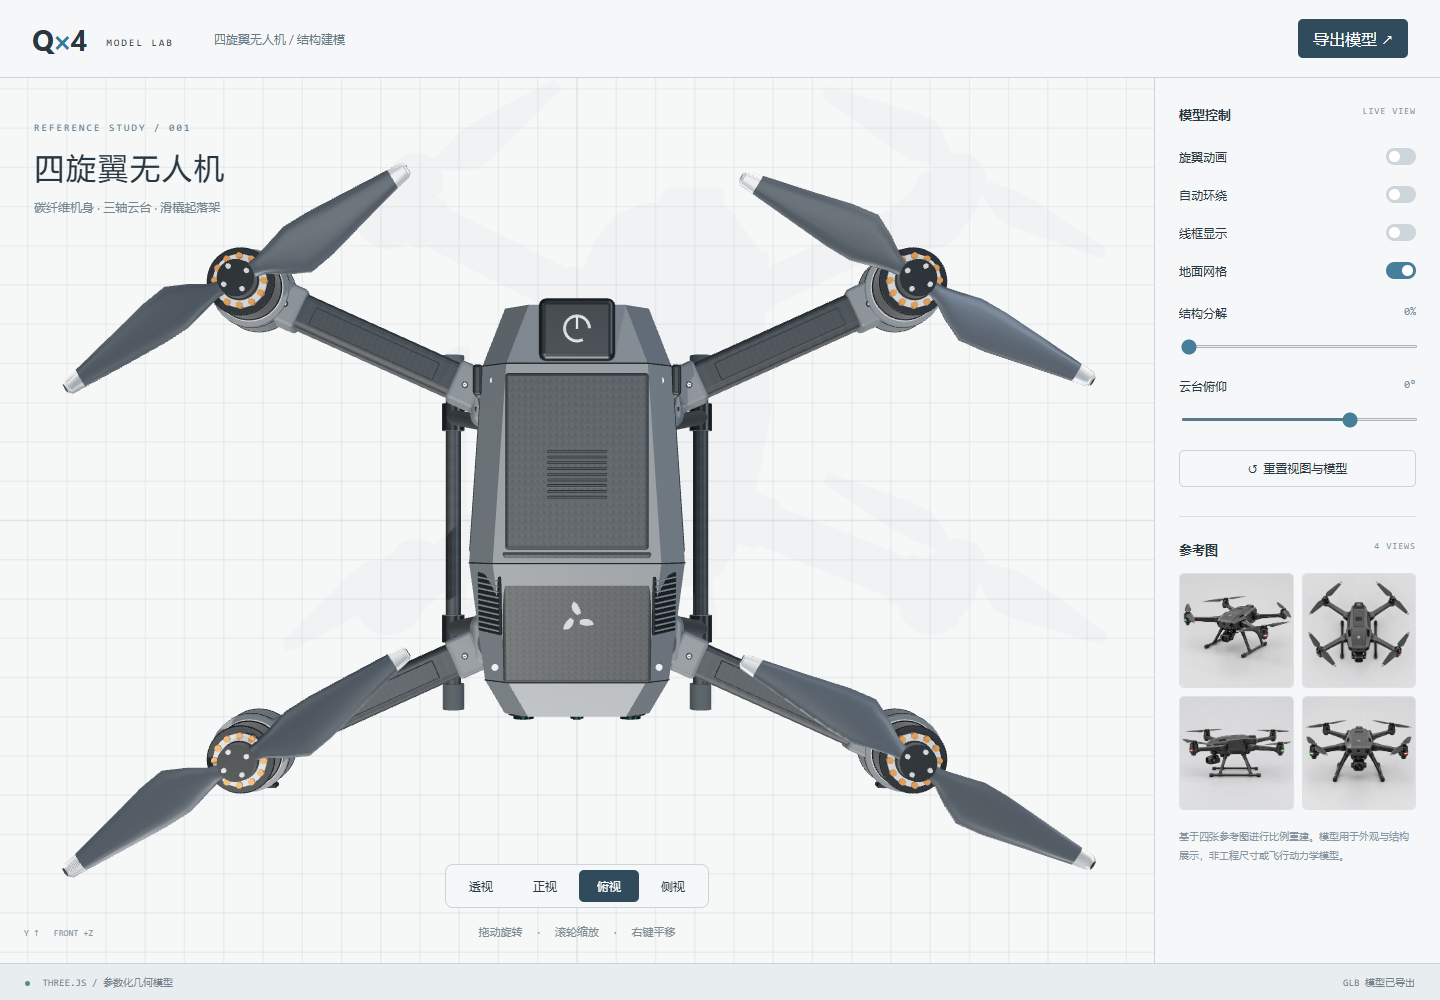
\includegraphics[width=.80\linewidth]{../top-preview.png}
\caption{俯视效果截图：四组旋翼、机身面板、散热结构与机臂布局。}
\end{figure}

\clearpage
\section{一个令人印象深刻的细节：航灯配色}
笔者尤其注意到，最终模型甚至修正了侧视参考图中左后方航灯的颜色：参考图的可见后侧航灯呈绿色，而模型将机体左侧的航灯统一为红色，右侧统一为绿色。从结果来看，这种处理遵循了“红左绿右”的配色原则，是一次令人印象深刻的细节修正。

这里的“左、右”以\textbf{无人机自身朝向}为准，而非屏幕左右。项目以 $Y$ 轴向上、$+Z$ 为机头方向，因此机体左侧对应 $+X$，右侧对应 $-X$。代码将 $+X$ 一侧设为红灯，$-X$ 一侧设为绿灯；从机头正面观察时，就会看到画面左侧为绿灯、右侧为红灯。对侧视参考图的左右判断，则依据其机头朝向及透视关系。

\begin{figure}[htbp]\centering
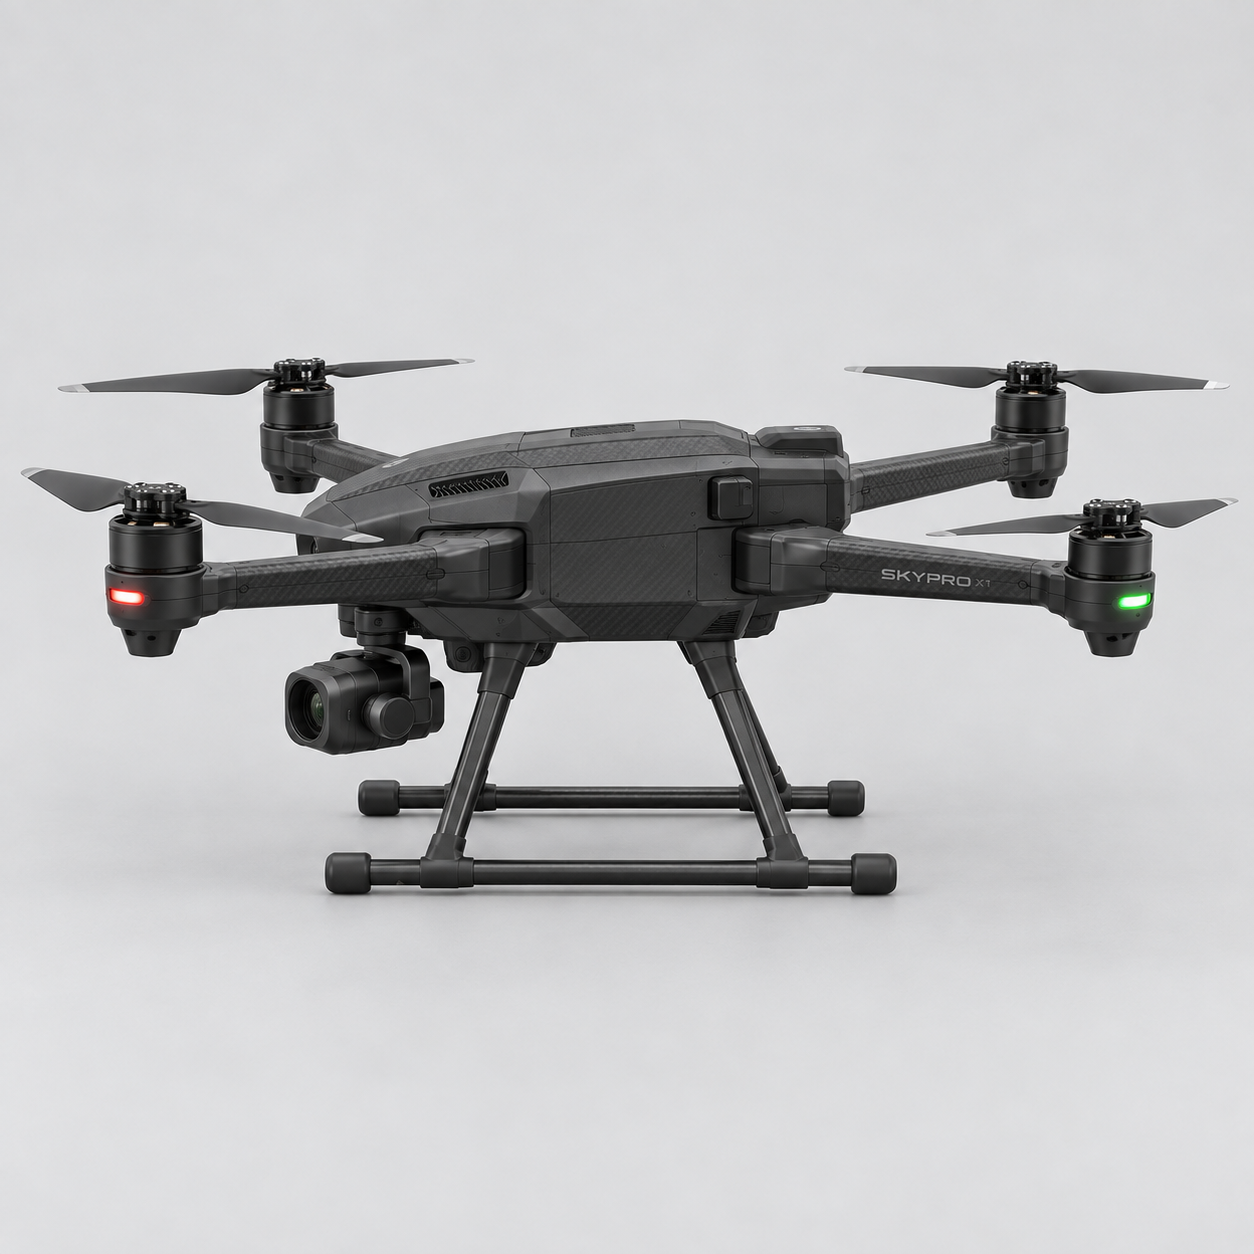
\includegraphics[width=.34\linewidth]{../figures/3.png}\hspace{.025\linewidth}
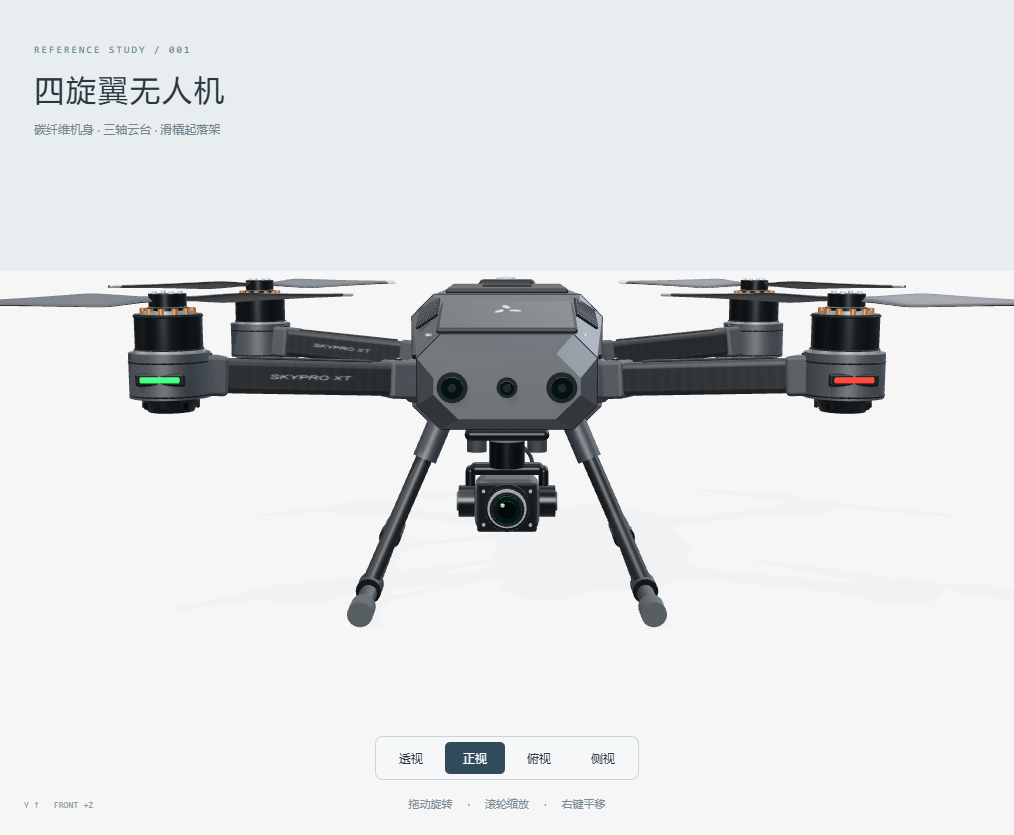
\includegraphics[width=.57\linewidth]{figures/front.png}
\caption{左：侧视参考图，可见前后航灯配色不同；右：模型正面截图，画面左绿右红，对应机体右绿左红。}
\end{figure}

这一结果体现了模型在配色一致性上的严谨。不过，现有对话记录没有直接说明其是否主动识别了参考图的航灯矛盾；能够确认的是最终代码和渲染结果确实采用了上述一致配色。本文将其作为结果层面的观察，而不推断模型未表达的内部判断过程。

\section{实现、验证与复现}
项目使用 Three.js 和 Vite。\texttt{src/drone.js} 负责整机与部件组织，\texttt{src/propeller.js} 负责桨叶几何，\texttt{src/main.js} 负责光照、相机、交互和导出。用户可以旋转、缩放和平移视图，切换透视、正视、俯视或侧视，控制旋翼动画、自动环绕、线框和网格，并通过滑块分解结构、调整云台俯仰。

实现过程中完成了生产构建、浏览器渲染与 GLB 导出检查；左右旋桨叶通过了网格边闭合性和有向体积检查。这些验证用于确认展示模型与导出流程可用，不等同于空气动力学验证。参考图没有尺寸标注，因此所有尺寸均为图片比例估算，未包含质量惯量、真实飞行动力学或控制系统。

\noindent 克隆仓库后，在项目根目录执行：
\begin{quote}\ttfamily
npm install\\
npm run dev
\end{quote}
打开终端给出的本地地址即可查看模型。执行 \texttt{npm run build} 可生成生产构建。导出 GLB 会保留当前结构分解状态与云台姿态；需要完整装配模型时，应先点击“重置视图与模型”。本文可在 \texttt{docs/} 目录下使用 XeLaTeX 编译两次。

\end{document}
